%*******10********20********30********40********50********60********70********80
%% ----------------------------------------------------------------
%% Thesis.tex -- MAIN FILE (the one that you compile with LaTeX)
%% ---------------------------------------------------------------- 

%% This template is based on Graduate Thesis written by Sunil Patel,
% (ho based it on the ecsthesis template) under the LaTeX Project Public License.
% which can be found here: http://latex-project.org/lppl/
% in the hope that it will be easier to use and to scale down to your needs
% by Simon Ternsjö in 2013-10



% INSTRUCTIONS:

% The meaning is not to edit this document much, but to fill in information 
% in the different files in the folders;
% Settings, Frontpages, Chapters, Appendices and possibly Files,
% as well as the file Bibliography.bib

% This template is easy to scale down to suite your need, 
% simply comment the input statements explained below


% Set up the document:
\documentclass[a4paper, 11pt, oneside]{Thesis}  % Use the "Thesis" style, based on the ECS Thesis style by Steve Gunn

% Add more package in Package.tex:
% Add your own packages here, 
% these existing packages can be removed if necessary
% not that more packages are imported in Thesis.cls, '
%  but those should not be changed if you don't know what you are doing...


\usepackage[utf8]{inputenc} % for writing other that basic characters
\usepackage{graphicx}
\usepackage{caption}
\usepackage{subcaption}



% Include any extra LaTeX packages required
\usepackage[square, numbers, comma, sort&compress]{natbib}  % Use the "Natbib" style for the references in the Bibliography
\usepackage{verbatim}  % Needed for the "comment" environment to make LaTeX comments
%5%\usepackage{vector}  % Allows "\bvec{}" and "\buvec{}" for "blackboard" style bold vectors in maths




% Use if you want:
%5%\graphicspath{Figures/}  % Location of the graphics files (set up for graphics to be in PDF format)
%5%\hypersetup{urlcolor=blue, colorlinks=true}  % Colours hyperlinks in blue, but this can be distracting if there are many links.

% Set your name, the title of the report and more in Administraitve.tex:
% This is where author, university, title and more is defined

% Personal information:
\newcommand{\myTitle}       {Infinite, procedural generated 3D world} % Thesis title goes here

% University information
\newcommand{\myUniversity}{Linköping University} %The Iniversity name goes here
\newcommand{\myGroup}{Horse and cats}
\newcommand{\myGroupWeb}{http://www.horseandcats.com)}

% can be left untouched, both:
\newcommand{\myDate}{\today}


%% ----------------------------------------------------------------
\begin{document}
\frontmatter      % Begin Roman style (i, ii, iii, iv...) page numbering


% Here the first pages are imported, you can find them in the Frontpages folder
% Files in the subfolder Fixed does not need to be edited.
% If you don't need any of these sections, simply comment, or delete, the input-row


%% All the pages before the chapters ------------------------------
\title{Infinite, procedural generated 3D worlds} % Title

\author{Lukas Berglin, Lukbe154\\
Ikshu Dutta, Iksdu821\\
Robin Silverhav Robsi807\\
Carl Stejmar, Carst056\\
Peter Thulin, Petth936}

\date{\today} % Date for the report

\maketitle % Insert the title, author and date

%\begin{figure}[h]
%\centering
%\includegraphics[scale=1.4]{3D_landscape}
%\label{3d_landscape}
%\end{figure}


\clearpage

% The Abstract Page
\clearpage 
\addtotoc{Abstract}  % Add the "Abstract" page entry to the Contents
\abstract{
    \addtocontents{toc}{\vspace{1em}}  % Add a gap in the Contents, 
                                        %for aesthetics
    
    %The Thesis Abstract is written here (and usually kept to just this page). 
    %The page is kept centered vertically so can expand into the blank space above the title too \ldots
    
    Abstract
    

    
}



\clearpage
\setstretch{1.3} % Reset the line-spacing to 1.3 for body text (if changed)
\pagestyle{fancy} % The page style headers have been "empty" all this time, 
                  % now use the "fancy" headers as defined before
\lhead{\emph{Contents}}  % Set the left side page header to "Contents"
\tableofcontents  % Write out the Table of Contents


\setstretch{1.3} % Reset the line-spacing to 1.3 for body text (if changed)
\pagestyle{fancy} % The page style headers have been "empty" all this time, 
                  % now use the "fancy" headers as defined before
\lhead{\emph{List of Figures}}  % left side page header to "List if Figures"
\listoffigures  % Write out the List of Figures


\clearpage  % Start a new page
\setstretch{1.3} % Reset the line-spacing to 1.3 for body text (if changed)
\pagestyle{fancy} % The page style headers have been "empty" all this time, 
                  % now use the "fancy" headers as defined before
\lhead{\emph{List of Tables}}  % left side page header to "List of Tables"
\listoftables  % Write out the List of Tables


\clearpage
\pagestyle{fancy} % The page style headers have been "empty" all this time, 
                  % now use the "fancy" headers as defined before
\setstretch{1.5} % Set the line spacing to 1.5, 
                 % this makes the following tables easier to read
\lhead{\emph{Abbreviations}}  % Set the left side page header to "Abbreviations"
\listofsymbols{ll}  % Include a list of Abbreviations (a table of two columns)
{
  % \textbf{Acronym} & \textbf{W}hat (it) \textbf{S}tands \textbf{F}or \\
   \textbf{LAH} & \textbf{L}ist \textbf{A}bbreviations \textbf{H}ere \\
   \textbf{OWL} & \textbf{O}rdinary \textbf{W}izarding \textbf{L}evel\\
}






%% The Body -------------------------------------------------------
\setstretch{1.3}  % Return the line spacing back to 1.3
\mainmatter	  % Begin normal, numeric (1,2,3...) page numbering
\pagestyle{fancy}  % Return the page headers back to the "fancy" style


% Include the chapters of the thesis, as separate files
% Just uncomment the lines as you write the chapters

%*******10********20********30********40********50********60********70********80

% For all chapters, use the newdefined chap{} instead of chapter{}
% This will make the text at the top-left of the page be the same as the chapter

\chap{Introduction}

Lorem ipsum dolor sit amet, consectetur adipiscing elit. Vivamus at pulvinar nisi. Phasellus hendrerit, diam placerat interdum iaculis, mauris justo cursus risus, in viverra purus eros at ligula. Ut metus justo, consequat a tristique posuere, laoreet nec nibh. Etiam et scelerisque mauris. Phasellus vel massa magna. Ut non neque id tortor pharetra bibendum vitae sit amet nisi. Duis nec quam quam, sed euismod justo. Pellentesque eu tellus vitae ante tempus malesuada. Nunc accumsan, quam in congue consequat, lectus lectus dapibus erat, id aliquet urna neque at massa. Nulla facilisi. Morbi ullamcorper eleifend posuere. Donec libero leo, faucibus nec bibendum at, mattis et urna. Proin consectetur, nunc ut imperdiet lobortis, magna neque tincidunt lectus, id iaculis nisi justo id nibh. Pellentesque vel sem in erat vulputate faucibus molestie ut lorem.

\section{A Section}

Quisque tristique urna in lorem laoreet at laoreet quam congue. Donec dolor turpis, blandit non imperdiet aliquet, blandit et felis. In lorem nisi, pretium sit amet vestibulum sed, tempus et sem. Proin non ante turpis. Nulla imperdiet fringilla convallis. Vivamus vel bibendum nisl. Pellentesque justo lectus, molestie vel luctus sed, lobortis in libero. Nulla facilisi. Aliquam erat volutpat. Suspendisse vitae nunc nunc. Sed aliquet est suscipit sapien rhoncus non adipiscing nibh consequat. Aliquam metus urna, faucibus eu vulputate non, luctus eu justo.

\subsection{A Subsection}

Donec urna leo, vulputate vitae porta eu, vehicula blandit libero. Phasellus eget massa et leo condimentum mollis. Nullam molestie, justo at pellentesque vulputate, sapien velit ornare diam, nec gravida lacus augue non diam. Integer mattis lacus id libero ultrices sit amet mollis neque molestie. Integer ut leo eget mi volutpat congue. Vivamus sodales, turpis id venenatis placerat, tellus purus adipiscing magna, eu aliquam nibh dolor id nibh. Pellentesque habitant morbi tristique senectus et netus et malesuada fames ac turpis egestas. Sed cursus convallis quam nec vehicula. Sed vulputate neque eget odio fringilla ac sodales urna feugiat.

\section{Another Section}

Phasellus nisi quam, volutpat non ullamcorper eget, congue fringilla leo. Cras et erat et nibh placerat commodo id ornare est. Nulla facilisi. Aenean pulvinar scelerisque eros eget interdum. Nunc pulvinar magna ut felis varius in hendrerit dolor accumsan. Nunc pellentesque magna quis magna bibendum non laoreet erat tincidunt. Nulla facilisi.

Duis eget massa sem, gravida interdum ipsum. Nulla nunc nisl, hendrerit sit amet commodo vel, varius id tellus. Lorem ipsum dolor sit amet, consectetur adipiscing elit. Nunc ac dolor est. Suspendisse ultrices tincidunt metus eget accumsan. Nullam facilisis, justo vitae convallis sollicitudin, eros augue malesuada metus, nec sagittis diam nibh ut sapien. Duis blandit lectus vitae lorem aliquam nec euismod nisi volutpat. Vestibulum ornare dictum tortor, at faucibus justo tempor non. Nulla facilisi. Cras non massa nunc, eget euismod purus. Nunc metus ipsum, euismod a consectetur vel, hendrerit nec nunc.

\LaTeX{} is great!

 % Introduction

%*******10********20********30********40********50********60********70********80

% For all chapters, use the newdefined chap{} instead of chapter{}
% This will make the text at the top-left of the page be the same as the chapter

\chap{Background Theory} % history of the jetpak

Lorem ipsum dolor sit amet, consectetur adipiscing elit. Vivamus at pulvinar nisi. Phasellus hendrerit, diam placerat interdum iaculis, mauris justo cursus risus, in viverra purus eros at ligula. Ut metus justo, consequat a tristique posuere, laoreet nec nibh. Etiam et scelerisque mauris. Phasellus vel massa magna. Ut non neque id tortor pharetra bibendum vitae sit amet nisi. Duis nec quam quam, sed euismod justo. Pellentesque eu tellus vitae ante tempus malesuada. Nunc accumsan, quam in congue consequat, lectus lectus dapibus erat, id aliquet urna neque at massa. Nulla facilisi. Morbi ullamcorper eleifend posuere. Donec libero leo, faucibus nec bibendum at, mattis et urna \cite{AWriter}. Proin consectetur, nunc ut imperdiet lobortis, magna neque tincidunt lectus, id iaculis nisi justo id nibh. Pellentesque vel sem in erat vulputate faucibus molestie ut lorem.

\begin{figure}
    \centering
    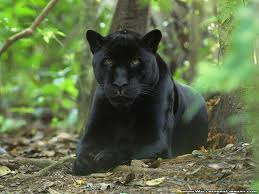
\includegraphics[scale=1, angle=0]{Files/panther.jpg}
    \caption[The panther]{A panther is always watching}
    \label{fig: jordan}
\end{figure}

Duis nec quam quam, sed euismod justo. Pellentesque eu tellus vitae ante tempus malesuada. Nunc accumsan, quam in congue consequat, lectus lectus dapibus erat, id aliquet urna neque at massa. Nulla facilisi. Morbi ullamcorper eleifend posuere. Donec libero leo, faucibus nec bibendum at, mattis et urna. Proin consectetur, nunc ut imperdiet lobortis, magna neque tincidunt lectus, id iaculis nisi justo id nibh. Pellentesque vel sem in erat vulputate faucibus molestie ut lorem.


\begin{figure}
        \centering
        \begin{subfigure}[b]{0.4\textwidth}
                \centering        %   l   b   r   t
                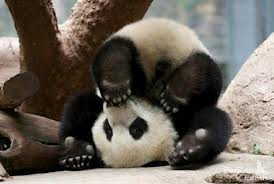
\includegraphics[trim=0.3cm 0cm 0cm 0cm, clip=true, 
                                width=\linewidth]
                                {Files/panda.jpg}
                \caption{Panda}
                \label{subfig: ff}
        \end{subfigure}
        ~ % for a little horisontal distance
        \raisebox{3cm}[\height][\depth]{$\Rightarrow$}
        \hspace{0.2mm} % for a little horisontal distance
        \begin{subfigure}[b]{0.4\textwidth}
                \centering
                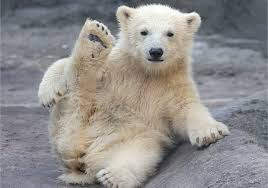
\includegraphics[trim=0cm 0cm 0cm 0cm, clip=true, 
                                width=\linewidth]
                                {Files/polarbear.jpg}
                \caption{Polar bear}
                \label{subfig: sf}
        \end{subfigure}
        \caption[The panda-polar bear relationship ]
                {It is not widely known that the panda becomes a polar bear 
                when dressing up in the winter camouflage suite \cite{AnExpert}}
        \label{fig: pentagram}
\end{figure}




 % Background Theory 

%*******10********20********30********40********50********60********70********80

% For all chapters, use the newdefined chap{} instead of chapter{}
% This will make the text at the top-left of the page be the same as the chapter

\chap{Development Method}

Tables are good \cite{ATraveler} which is shown in \ref{table: you} and 
\ref{table: whether}!
\begin{table}[ht] 
    \centering 
    \begin{tabular}{|r|l|}
        \hline
        7C0 & hexadecimal \\
        3700 & octal \\ \cline{2-2}
        11111000000 & binary \\
        \hline \hline
        1984 & decimal \\
        \hline
    \end{tabular}
    \caption[You-table]{Table for you}
    \label{table: you} % is used to refer this table in the text 
\end{table} 

\begin{table}[ht] 
    \centering 
    \begin{tabular}{ | l | l | l | p{5cm} |}
        \hline
        Day & Min Temp & Max Temp & Summary \\ \hline
        Monday & 11C & 22C & A clear day with lots of sunshine. \\ \hline
        Tuesday & 9C & 19C & Cloudy with rain, \\ \hline
        Wednesday & 10C & 21C & Rain will still linger for the morning.\\
        \hline
    \end{tabular}
    \caption[Weather table]{Whether table for tomorrow}
    \label{table: whether} 
\end{table} 


 % Experimental Setup

%\input{Chapters/Chapter4} % Experiment 1

%\input{Chapters/Chapter5} % Experiment 2

%\input{Chapters/Chapter6} % Results and Discussion

%\input{Chapters/Chapter7} % Conclusion



%% Appendices -----------------------------------------------------
\addtocontents{toc}{\vspace{2em}} % Add a gap in the Contents, for aesthetics
\lhead{\emph{Appendices}}  % Change the left side page header to "Appendices"
\appendix % Cue to tell LaTeX that the following 'chapters' are Appendices

\chap{An Appendix}

Lorem ipsum dolor sit amet, consectetur adipiscing elit. Vivamus at pulvinar nisi. Phasellus hendrerit, diam placerat interdum iaculis, mauris justo cursus risus, in viverra purus eros at ligula. Ut metus justo, consequat a tristique posuere, laoreet nec nibh. Etiam et scelerisque mauris. Phasellus vel massa magna. Ut non neque id tortor pharetra bibendum vitae sit amet nisi. Duis nec quam quam, sed euismod justo. Pellentesque eu tellus vitae ante tempus malesuada. Nunc accumsan, quam in congue consequat, lectus lectus dapibus erat, id aliquet urna neque at massa. Nulla facilisi. Morbi ullamcorper eleifend posuere. Donec libero leo, faucibus nec bibendum at, mattis et urna. Proin consectetur, nunc ut imperdiet lobortis, magna neque tincidunt lectus, id iaculis nisi justo id nibh. Pellentesque vel sem in erat vulputate faucibus molestie ut lorem.

Quisque tristique urna in lorem laoreet at laoreet quam congue. Donec dolor turpis, blandit non imperdiet aliquet, blandit et felis. In lorem nisi, pretium sit amet vestibulum sed, tempus et sem. Proin non ante turpis. Nulla imperdiet fringilla convallis. Vivamus vel bibendum nisl. Pellentesque justo lectus, molestie vel luctus sed, lobortis in libero. Nulla facilisi. Aliquam erat volutpat. Suspendisse vitae nunc nunc. Sed aliquet est suscipit sapien rhoncus non adipiscing nibh consequat. Aliquam metus urna, faucibus eu vulputate non, luctus eu justo.

Donec urna leo, vulputate vitae porta eu, vehicula blandit libero. Phasellus eget massa et leo condimentum mollis. Nullam molestie, justo at pellentesque vulputate, sapien velit ornare diam, nec gravida lacus augue non diam. Integer mattis lacus id libero ultrices sit amet mollis neque molestie. Integer ut leo eget mi volutpat congue. Vivamus sodales, turpis id venenatis placerat, tellus purus adipiscing magna, eu aliquam nibh dolor id nibh. Pellentesque habitant morbi tristique senectus et netus et malesuada fames ac turpis egestas. Sed cursus convallis quam nec vehicula. Sed vulputate neque eget odio fringilla ac sodales urna feugiat.

Phasellus nisi quam, volutpat non ullamcorper eget, congue fringilla leo. Cras et erat et nibh placerat commodo id ornare est. Nulla facilisi. Aenean pulvinar scelerisque eros eget interdum. Nunc pulvinar magna ut felis varius in hendrerit dolor accumsan. Nunc pellentesque magna quis magna bibendum non laoreet erat tincidunt. Nulla facilisi.

Duis eget massa sem, gravida interdum ipsum. Nulla nunc nisl, hendrerit sit amet commodo vel, varius id tellus. Lorem ipsum dolor sit amet, consectetur adipiscing elit. Nunc ac dolor est. Suspendisse ultrices tincidunt metus eget accumsan. Nullam facilisis, justo vitae convallis sollicitudin, eros augue malesuada metus, nec sagittis diam nibh ut sapien. Duis blandit lectus vitae lorem aliquam nec euismod nisi volutpat. Vestibulum ornare dictum tortor, at faucibus justo tempor non. Nulla facilisi. Cras non massa nunc, eget euismod purus. Nunc metus ipsum, euismod a consectetur vel, hendrerit nec nunc. % Appendix Title

%\input{Appendices/AppendixB} % Appendix Title

%\input{Appendices/AppendixC} % Appendix Title


%% Bibliography ---------------------------------------------------
\backmatter % Cue to tell LaTeX that the following 'chapters' are Bibliography
\label{Bibliography}
\lhead{\emph{Bibliography}}  % left side page header to "Bibliography"
\bibliographystyle{unsrtnat}  % Use the "unsrtnat" BibTeX style for formatting the Bibliography

\begingroup
    \raggedright
    \sloppy
    \bibliography{Bibliography}  % The references (bibliography) information are stored in the file named "Bibliography.bib"
\endgroup 


\end{document}  % The End
%% ----------------------------------------------------------------